\nonstopmode
\documentclass{beamer}
\usepackage{tikz}

\usetikzlibrary{plotmarks}
\usepackage{pgfplots}
\pgfplotsset{compat=1.5}

\usepackage{shellesc}
\usepackage{minted}
\setminted[python]{tabsize=2, linenos=true, breaklines=true}

\usepackage{multirow}
\usepackage{booktabs}
\usepackage{pbox}
\renewcommand{\arraystretch}{1.5}

\usepackage[binary-units]{siunitx}

\usepackage{ulem}

\usepackage{appendixnumberbeamer}

\title{Op zoek naar een goede afstelling van de fiets\\
met een genetisch algoritme}

\author{Michiel Vos}

\date{23 september 2016}

\begin{document}

\begin{frame}
  \titlepage
\end{frame}

\begin{frame}
  \frametitle{Doel}
  \begin{itemize}
      \item Michiel
      \item Theorie
      \item Praktijk (bonus)
  \end{itemize}
\end{frame}

\begin{frame}
  \frametitle{Probleem}
  \begin{itemize}
      \item Fiets 
      \item Veel onderdelen
      \item Optimale afstelling (helm, houding)
  \end{itemize}
\end{frame}

\begin{frame}
  \frametitle{Opties}
  \begin{itemize}
      \item Brute kracht
      \item Gretig algoritme
      \item Genetisch algoritme
  \end{itemize}
\end{frame}

\begin{frame}
  \frametitle{Genetich algoritme}
  \begin{itemize}
      \item Intro
  \end{itemize}
\end{frame}

\begin{frame}
  \frametitle{Onderdelen}
  \begin{center}
    
\includegraphics[width=200px]{michiel.png}
  \end{center}
\end{frame}

\begin{frame}
  \frametitle{Individu}
  \begin{itemize}
      \item DNA
  \end{itemize}
  \begin{tabular}{|M | M | M|}
              \hline
              1 0 1 0 1 0 \\ \hline
              1 0 1 0 1 0 \\
              \hline
            \end{tabular}
\end{frame}

\begin{frame}
  \frametitle{Fitness}
  \begin{itemize}
      \item Vaste omstandigheden
  \end{itemize}
\end{frame}

\begin{frame}
  \frametitle{Generatie 0}
  \begin{itemize}
      \item Michiel
  \end{itemize}
\end{frame}

\begin{frame}
  \frametitle{Selectie}
  \begin{itemize}
      \item Michiel
  \end{itemize}
\end{frame}

\begin{frame}
  \frametitle{Combinatie}
  \begin{itemize}
      \item Crossover
  \end{itemize}
\end{frame}

\begin{frame}
  \frametitle{Mutatie}
  \begin{itemize}
      \item Michiel
  \end{itemize}
\end{frame}

\begin{frame}
  \frametitle{Mutatie}
  \begin{itemize}
      \item Michiel
  \end{itemize}
\end{frame}

\begin{frame}
  \frametitle{Vragen?}
  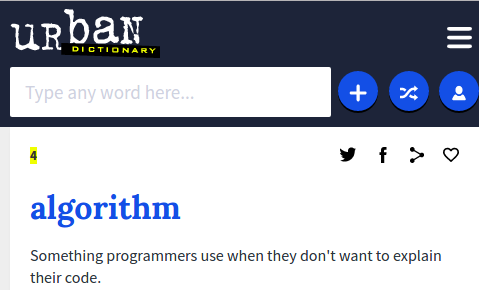
\includegraphics[width=300px]{algorithm.png}
\end{frame}

\end{document}
